\documentclass[preprint2,times,tighten]{aastex6}

%\pdfoutput=2 %for arXiv submission
\usepackage{amsmath,amstext}
\usepackage[figure,figure*]{hypcap}
\usepackage{newtxmath} %use times font for math


\newcommand{\teff}{$\tau_\mathrm{eff}$\space}
\newcommand{\lya}{Ly$\alpha$\space}
\newcommand{\kms}{km~s$^{-1}$\space}
\newcommand{\zem}{$\mathrm{z_{med}}$\space}
\newcommand{\hiz}{$\mathrm{z_{high}}$\space}
\newcommand{\loz}{$\mathrm{z_{low}}$\space}
\newcommand{\rchi}{$\chi^{2}_\mathrm{reduced}$}



\begin{document}

\title{Effective Opacity of the Intergalactic Medium from Galaxies}

\author{ Jose S. Monzon\altaffilmark{1},
J. Xavier Prochaska\altaffilmark{1,2}, Khee-Gan Lee\altaffilmark{2}}
\altaffiltext{1}{University of California, Santa Cruz; 1156 High St., Santa Cruz, CA 95064, USA}
\altaffiltext{2}{Kavli Institute for the Physics and Mathematics of the Universe (Kavli IPMU);The University of Tokyo; 5-1-5 Kashiwanoha, Kashiwa, 277-8583, Japan}


\begin{abstract}
We measure the effective opacity of the Intergalactic Medium (IGM) with the composite spectra of 202 Lyman-Break Galaxies (LBGs) in the range of $2 \leq z \leq 3$. Our spectra were taken from the COSMOS Lyman-Alpha Mapping And Tomographic Observations (CLAMATO) survey derived from the Low Resolution Imaging Spectrometer (LRIS) on the W.M. Keck I telescope. The Spectral Energy Distribution (SEDs) models we fit to our spectra are composed of simple stellar populations from the StarBurst99 data package. We measure the effective opacity (\teff) for every wavelength bin in our selection of the \lya forest and fit our distribution with an analytic power-law function. We find that scale factor and power-law index measurements of A = $0.158 \pm 0.007$  and B = $0.493 \pm 1.114$ (respectively) give a minimum \rchi = 1.941 with 86 degrees of freedom. Though our measurements generally agree with the most recent and careful studies from high-resolution spectra of both Quasi-Stellar Objects (QSOs) and galaxies, we report \teff values that are significantly scattered in our redshift range ($2.03 \leq z \leq 2.46$) and therefore poorly constrain the power-law index of our analytic fit. We present our estimate of the IGM's effective opacity evolution and present measurements that extend to the lowest redshifts that have been directly measured with galaxies.
\end{abstract}

\keywords{keywords --- Intergalactic Medium, Effective Opacity, Lyman Break Galaxy}
 

\section{Introduction}%%%%%%%%%%%%%%%%%%%%%%%%%%%%%%%%%%%%%%%%%%%%%%%%%%%%%%%%
\label{sec:intro}

The Intergalactic Medium (IGM) is a diffuse gas, mainly consisting of ionized hydrogen and helium, that permeates the space left by galaxy systems in the large scale cosmic web. The gas is highly ionized by the extragalactic ultraviolet background (EUVB) radiation field and takes the form of a diffuse, $T\sim 10^4$K plasma. It is, however, a trace neutral fraction of hydrogen gas ($\chi_\mathrm{HI}$) that is responsible for absorbing and attenuating the radiation from the EUVB and producing the \lya forest. (see \cite{McQuinn_2016} for a review). Studies on the \lya forest have meshed well with the theoretical constructs as it is the IGM, and not the galaxies it surrounds, that governs the large scale structure of the universe. It is considered one of the most powerful cosmological probes as it holds the majority of baryons at all epochs \citep{2007ApJ...662...72B} 

\cite{1965ApJ...142.1633G} were the first to discern that a universe filled with neutral hydrogen (HI) would be opaque in the UV, especially at higher redshifts where HI is densest. Analyzing the spectrum of any distant, rest-frame, UV object, directly points to a fluctuating and photo-ionized gas that at a given redshift, varies considerably from sight-line to sight-line. If analyzed, these variations in individual spectra can place statistical constraints on properties like density, temperature and composition and if sampled across the different redshifts, indicate the evolution of the IGM. A solid understanding of the physical state of the IGM allows for subsequent research investigating galaxy formation, the epoch of reionization, and ultimately the constraints on our leading cosmological theories.

Studies of the physical properties of the IGM have primarily come from the analysis of the mean optical depth of HI ($\tau$) observed in the spectra of distant Quasi-Stellar Objects (QSO's) \citep{prochaska_direct_2009, 2007ApJ...662...72B, faucher-giguere_direct_2008, kirkman_h_2005}. The emission of a QSO peaks in the UV because they are powered by accretion disks surrounding active galactic-nuclei (AGN) \citep{meiksin_physics_2009}. As the QSO's radiation traverses the space between galaxies, a series of absorption lines populate the rest-frame spectrum blueward of 1215\AA. Because the IGM is inhomogenous, photons from the same coordinates generally interact with the intervening gas at the different redshifts, causing absorption features across a multitude of wavelengths; the \lya forest. For a sufficiently far object, $z > 5$, the absorption lines become so saturated, that almost no flux is observed within the 1070-1170\AA \space range \citep{prochaska_hi_nodate}. This is because the attenuation of an object's spectra is dependant on $N_{HI}$ in the local IGM, and therefore is more effectively attenuated where the IGM is the densest. \citep{mcdonald_lyman-alpha_2006}. 

One can directly measure values describing the attenuation from the spectra of distant objects by estimating the continuum without any absorption, a process that becomes increasingly difficult at higher redshifts \citep{kirkman_h_2005}. However, the phenomena that creates the \lya forest is not exclusive to QSOs, and can be observed in the spectra of any distant UV-emmiting source. In fact, the EUVB is thought to be dominated by a numerous population of faint star forming galaxies at $z \gtrsim 3$ \citep{prochaska_direct_2009}. We set out to measure the effective opacity, \teff, using the spectra of Lyman-Break Galaxies (LBGs). We measure \teff by exploiting the high number density of high magnitude LBGs in the foreground ($2 <z< 3$) IGM \citep{lee_first_2018}. 

LBGs are star forming galaxies whose emissions also peak in the UV and visible ranges. They are selected based on their emission blueward of \lya in a given filter set. They contribute to the EUVB and aid in the ionization of the IGM because they harbour young and massive stars. Recently, \cite{thomas_vimos_2017} highlighted the importance of understanding the average IGM transmission not only for describing the properties of the intervening gas, but how that might affect the standard selection techniques for large samples of high-redshift galaxies \citep{steidel_spectroscopic_1996}.
\cite{thomas_vimos_2017}, like \cite{faucher-giguere_direct_2008, becker_refined_2013}, manages to investigate a wide range of redshift values from $2.5 < z < 5.5$ 

We follow the example of \cite{thomas_vimos_2017}, deviating from the common practices concerning the analysis of the \teff in that we use roughly 250, low-resolution and low S/N galaxy spectra as our as our sample. The main innovation of this work however is that we measure \teff using the spectra of objects found at $z < 2.5$. We hope to uncover any diversity in the measurements of \teff compared to other authors and contribute to working knowledge of how this opacity scales at these "lower" redshifts.

In the following sections we discuss: [2] the CLAMATO data sample [3] our methodologies for creating composite spectra, [4] fitting SEDs to our composite spectra, [5] the analysis of the modelled SED compared with our composite spectra [6] a discussion on this work’s findings. Throughout the paper, we adopt a concordance $\Lambda$CDM cosmology with $\Omega_{\Lambda}$ = 0.7, $\Omega_{m}$ = 0.3 and h = 0.7.


%%%%%%%%%%%%%%%%%%%%%%%%%%%%%%%%%%%%%%%%%%%%%%%%%%%%%%%%
\section{CLAMATO Sample Selection}
\label{sec:selection}

Our sample of galaxies was drawn from the 2016 and 2017 COSMOS Lyman-Alpha Mapping And Tomographic Observations (CLAMATO), which is conducted with the Low Resolution Imaging Spectrometer (LRIS) on W.M. Keck I telescope \citep{LRIS}. CLAMATO is designed to systematically observe faint star-forming galaxies from $2 \leq z \leq 3$, at high area densities \citep{lee_first_2018, lee_observational_2014}. CLAMATO's main goal is to map the \lya forest tomography of the foreground IGM. Because LBGs dominate the foreground UV luminosity function at g $\sim$ 23 \citep{reddy_multi-wavelength_2008}, \cite{lee_observational_2014} use them almost exclusively for their 3D tomographic reconstruction and analysis.

CLAMATO is the not the first survey with the goal of gauging the large scale structures of the IGM, so an area of the sky that is well studied was selected. The COSMOS field \citep{scoville_cosmic_2007} is in the Northern Hemisphere and spans 2 square degrees. It offers a large selection of g-band star forming galaxies, covers a significant scale in the transverse direction ($\sim$ 10Mpc) and has measurements of photometric/spectroscopic redshifts for the objects in the COSMOS survey. The target selection procedure depends on the initial prioritization based on redshift, magnitude and probability of success, and the subsequent slit mask designs \citep{lee_first_2018}. 

\begin{figure*}[ht]
    \begin{center}
    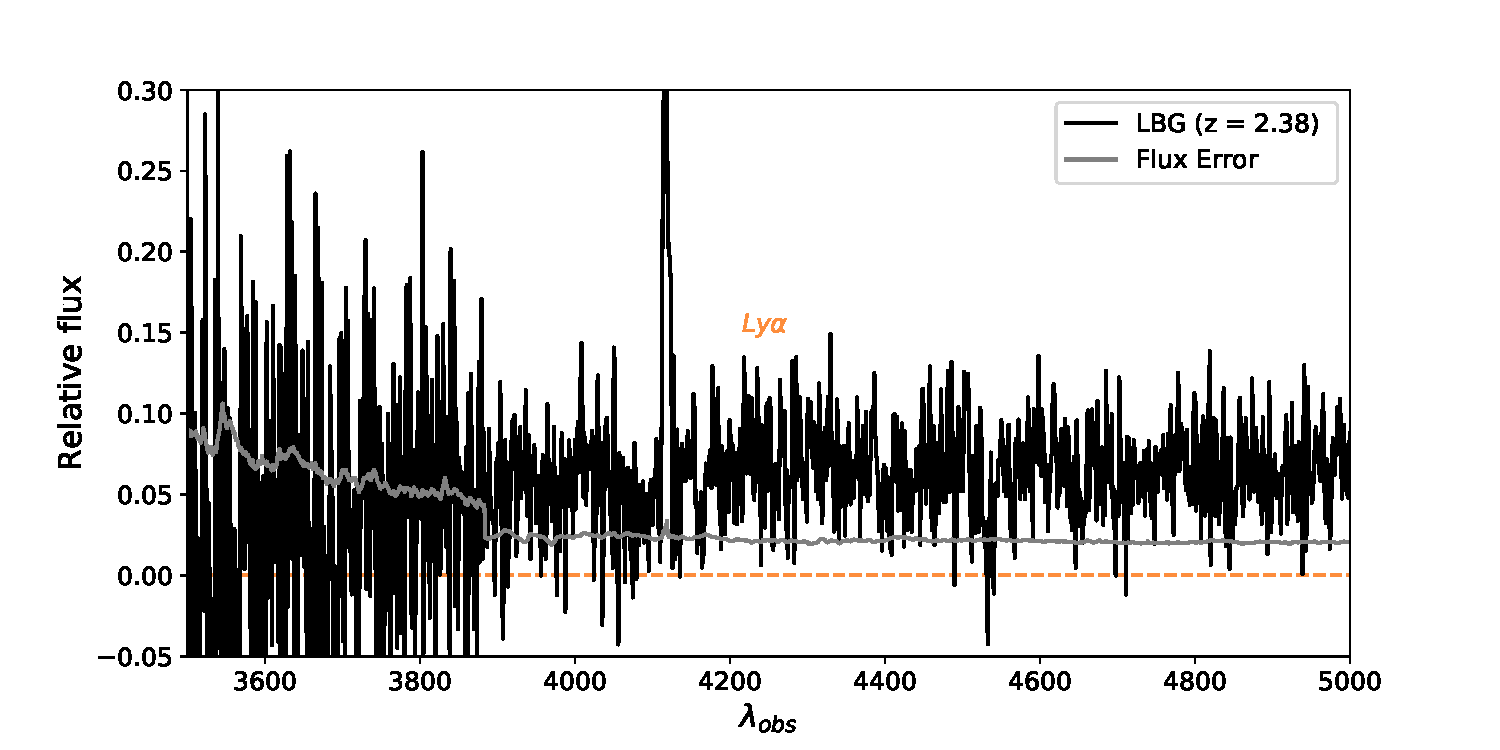
\includegraphics[scale=.5]{exspec.pdf}
    \caption{An example spectrum of a Lyman Break Galaxy from the CLAMATO survey. This is a well behaved representation of the spectra that fit our criteria. An error spectrum (shown in grey) is reported with each object in the reduced CLAMATO data set. The spectrum is quite noisy, with the only clear emission feature as \lya. Blueward of \lya, where our data tends to be noisiest, is where we measure \teff.}
    \label{fig:exspec}
    \end{center}
\end{figure*}


Observations for the CLAMATO surveys for 2014 - 2017 lasted a total of 15.5 nights of which about 60 hrs were spent on sky with typical total exposure time per object lasting $\sim$ 9000s. LRIS was configured with the 600/4000 grism to achieve an approximate resolution R $\equiv \lambda/\Delta\lambda \approx 1000$ with 1$"$ slits between the observer-frame wavelengths of 3700A and 4400A on its Blue channel. As expected with such faint and distant sources and an average seeing of 0.7$"$, our spectra were quiet noisy (S/N $<$ 3 per $\AA$). The data were then processed using the LowRedux routines from the XIDL software package \footnote{http://www.ucolick.org/$\sim$xavier/LowRedux}. To help extract fainter sources, after the standard flat fielding and sky subtraction, the authors co-added 2D individual exposures and then traced the corresponding 1D spectra. 

The CLAMATO team gave confidence ratings from 0-4 in identifying redshift for each source, 0 being no attempt all (normally reserved for corrupted data) and 4 being high confidence based on multiple lines. \cite{lee_first_2018} reports that 66\% of the objects in the sample had confidence ratings greater $> 3$, because they filled spare slit space with low priority sources that often yielded spectra too noisy to identify. 95\% of the objects with confidence ratings greater 3, were identified as galaxies using LBG templates from \cite{shapley_rest-frame_2003}, while the other 5\%, were distinguished as broad-line quasars. For a more detailed outline of the selection algorithm, instrument specifications and preliminary data reduction please see \cite{lee_first_2018}. 


\section{Composite Spectrum}%%%%%%%%%%%%%%%%%%%%%%%%%%%%%%%%%%%%%%%%%%%%%%%%%%%%%%%%
\label{sec:composite}

\teff is the \textit{effective} opacity of the IGM because it is measured by averaging the opacity from several different sight-lines. Measuring the opacity, $\tau$, from an individual object's spectrum, would yield a single (and therefore insufficient for our purposes) illustration of an inhomogeneous IGM. We measure \teff using a composite or "stacked" spectrum, which is essentially an average of flux values, per given wavelength. Alternatively, we could have measured the opacity from several different spectra, and then averaged, to yield \teff. There are two main justifications for why chose to average our data before measuring the opacity of the IGM: 1) For small redshift variations, the observed continua of LBGs (or QSOs) are more or less consistent, so a composite spectrum can be modeled by a single SED. 2) Stacking improves the S/N of the data which is necessary because the distant background sources we observe have large scatter in their flux values.

\subsection{Composite Sample}
\label{subsec:reduction}

To account for the fact that we are sampling the IGM with sight-lines corresponding to objects that are not at the same redshift, we organize our spectra into small redshift bins of $\Delta z = 0.25$. That way, the composites' median distance value, \zem, will be approximately at the center of the bin, allowing us to measure \teff per pixel in the \lya forest without bias. In total, there are 566 objects in the $2.0 \leq z \leq 3.0$ interval but the majority of our galaxies lie within the $2.25 < z < 2.75$ interval (see figure \ref{fig:clamatohist}). We only used the majority interval because the bins to either side of it (with the same $\Delta$z), would not have enough spectra to create an adequate stack. We split our latter interval into two redshift bins: \loz from $2.25 < z < 2.50$ and from \hiz from $2.50 < z < 2.75$. The \loz bin contains 210 galaxies and the \hiz bin has 197, for a combined total of 407 galaxies.


\begin{figure}[ht]
    \begin{center}
    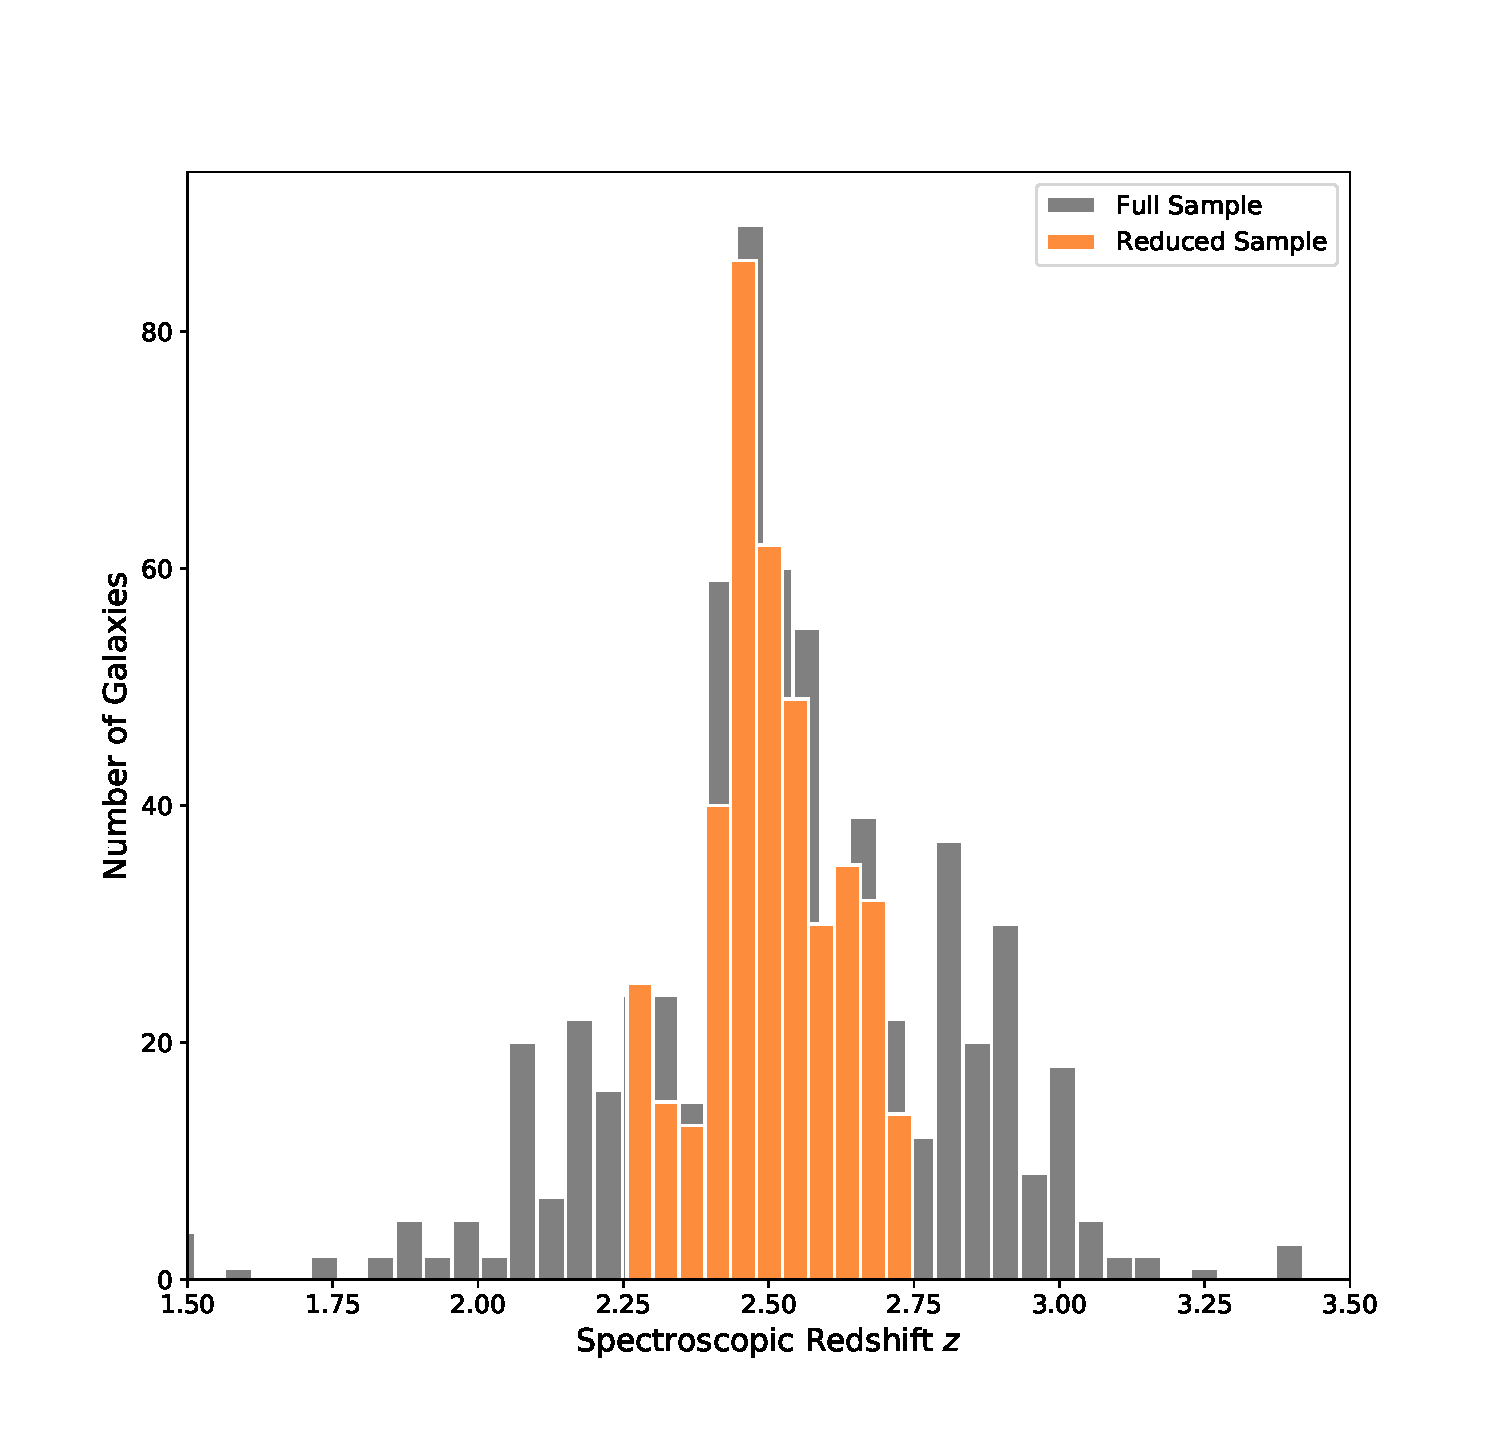
\includegraphics[width=\columnwidth]{clamatohist.pdf}
    \caption{The CLAMATO sample vs the selection we use to create our composites. The orange histogram includes both bins (\loz \& \hiz).}
    \label{fig:clamatohist}
    \end{center}
\end{figure}

For the 144 objects whose spectra extend blueward of the rest frame Lyman Limit (LL), we exclude those with fluxes outside of $\pm 0.2\sigma$ since this probably indicates bad fluxing or sky subtraction (see figure \ref{fig:ll_cut}). We further cut down our sample by imposing a blanket S/N limit, using the mean flux value (per angstrom) in the wavelength range of 1260-1304\AA. We found that a cut-off S/N value of = 1.5 excluded the poorest spectra without discarding the majority of an already noisy data sample (see figure \ref{fig:noise_scatter}). After these two cuts, we were left with 134 in \loz bin and 126 in \hiz bin; roughly 60\% of the spectra in both bins. The \loz bin has a median redshift value of 2.442 and a standard deviation of .059. The \hiz bin has a median redshift value of 2.606 and a standard deviation of .067

\begin{figure}[ht]
    \begin{center}
    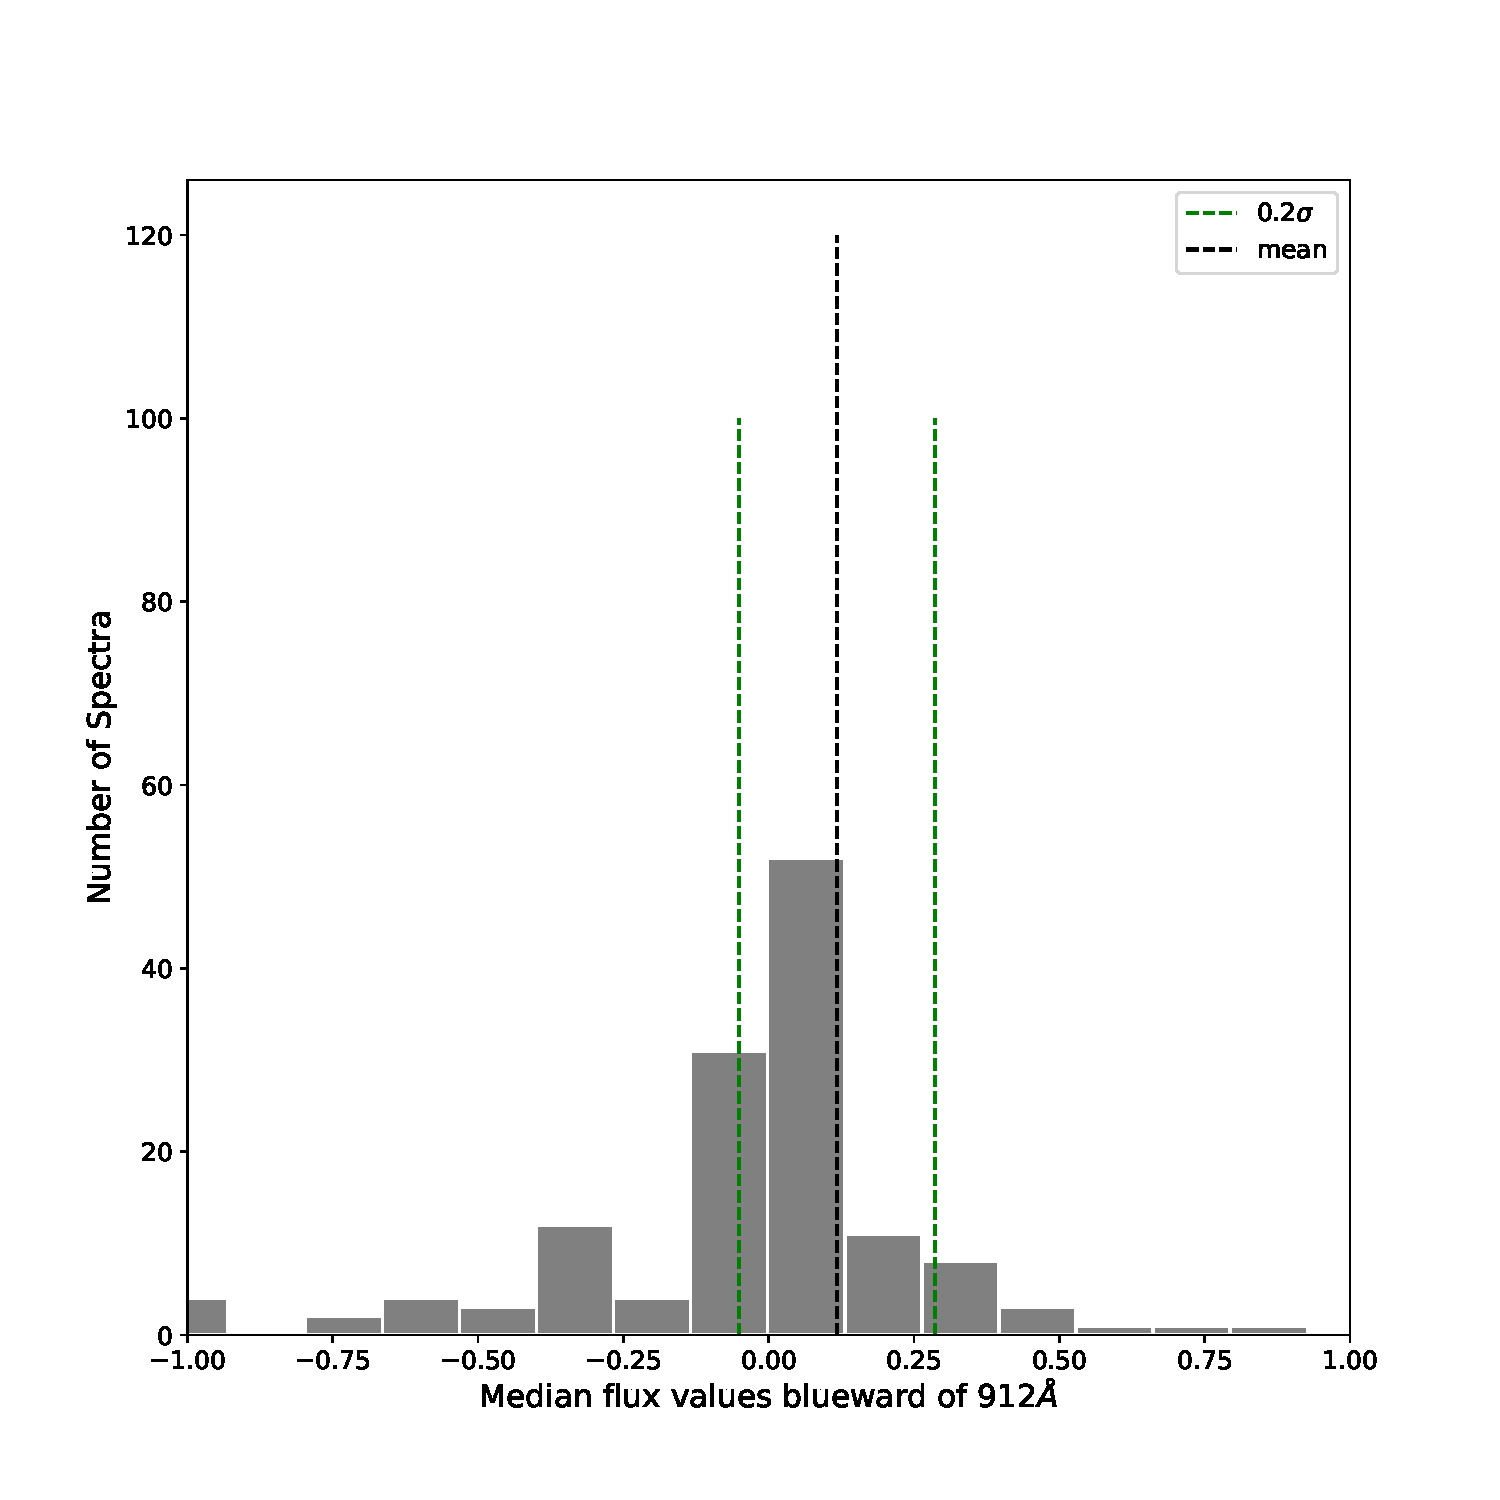
\includegraphics[width=\columnwidth]{ll_cut.pdf}
    \caption{144 spectra were selected in this sample because they extended blue-ward of the Lyman Limit. Only 50\% of the median flux values are within the $\pm 0.2\sigma$ cut-off. We cut our sample aggressively because, if included in a stack, these spectra would skew the blue side of the continuum nonphysically.}
    \label{fig:ll_cut}
    \end{center}
\end{figure}

\begin{figure}[ht]
    \begin{center}
    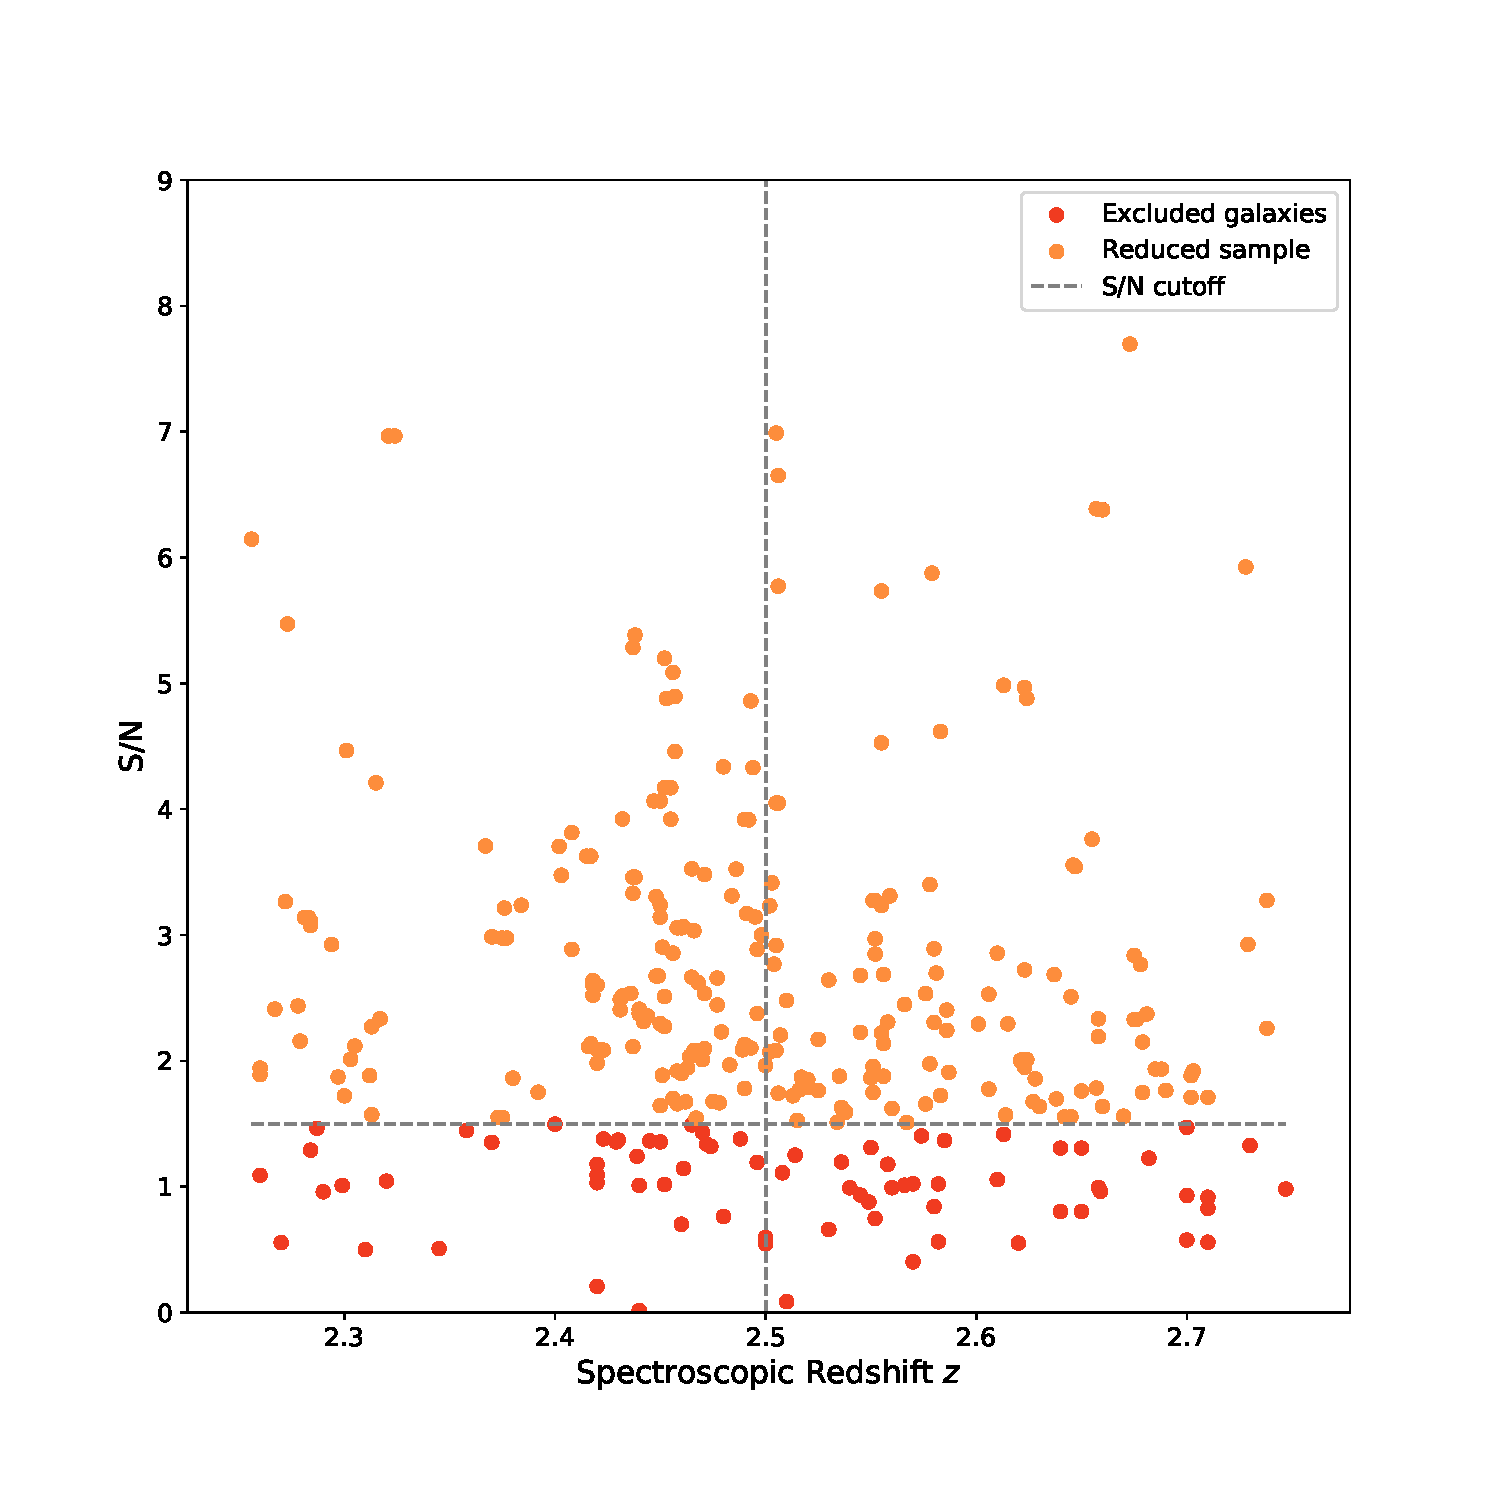
\includegraphics[width=\columnwidth]{noise_scatter.pdf}
    \caption{A scatter plot of our data sample for both bins: \loz \& \hiz. The x-axis measures spectroscopic redshift as measured by the CLAMATO survey, and the y-axis is S/N calculated in the same wavelength interval as the normalization 1260-1304\AA \citep{faucher-giguere_direct_2008}. The red objects have been excluded by S/N cut. The dotted vertical line separates the two bins.}
    \label{fig:noise_scatter}
    \end{center}
\end{figure}


\subsection{Stacking}
\label{subsec:stack}

The process that follows describes what we did to individual spectra in our high quality sample, before stacking them. [1] To correct extinction from our own interstellar medium (ISM), we passed the spectrum through a dereddening process based on the 3D Sky Map from \cite{2018MNRAS.478..651G}. The Sky Map, given an object's coordinates, reports $E(B-V)$ extinction values for the Milky Way which we applied to the flux arrays of our spectrum using the the reddening curve from \cite{calzetti_dust_2000}. [2] We normalized using values redward of \lya, where there is no absorption features due to the IGM or ISM, using the median of flux values in between the two SiII lines from 1260-1304\ \citep{faucher-giguere_direct_2008}. [3] We trimmed the edges of the spectrum, as we were only concerned with the values between $\lambda_{\rm rest} \approx 1050-1400$\AA.[4] We shifted the the wavelength array to the rest frame, using the redshift values measured by CLAMATO, and rebinning to a velocity dispersion of 300 km/s per pixel.

Only then did we stack the spectra by carrying out an unweighted, arithmetic mean of the flux per wavelength. We chose not to weigh the spectra to better reduce cosmic variance in the \lya forest \citep{becker_refined_2013}. Though the stacking process improved our S/N roughly as the $\sqrt{\textit{N}}$ (where \textit{N} is the number of spectra in the stack), leaving us at S/N $\sim$ 11 (in the same 1260-1304\AA range) the composites remained quite noisy at the edges.

\subsection{Bootstrapping}
\label{subsec:bootstrap}

To asses error in \teff, we used a bootstrapping approach that follows the example of \cite{worseck_giant_2014}. Our primary source of error comes from sample variance within the composite and not from the S/N values of each individual spectrum. For each redshift bin, the process is as follows: [1] We chose a random selection of spectra (that allowed for duplicates) from our composite sample [2] We stacked the random selection in the same way as detailed above for creating the original composite [3] We repeated the first two steps to generate 10,000 randomized composites [4] We subtracted the original composite from each of the randomized stacks [5] We compiled the randomized stacks into an $I x J$ matrix where $I$ = 10,000 and $J$ is the length of our wavelength array $\sim 1000$ [6] We dotted that matrix with its transpose and defined the diagonal of that product to be the error spectrum $\sigma_{f}$ for the original composite.

\begin{figure*}[ht]
    \centering
    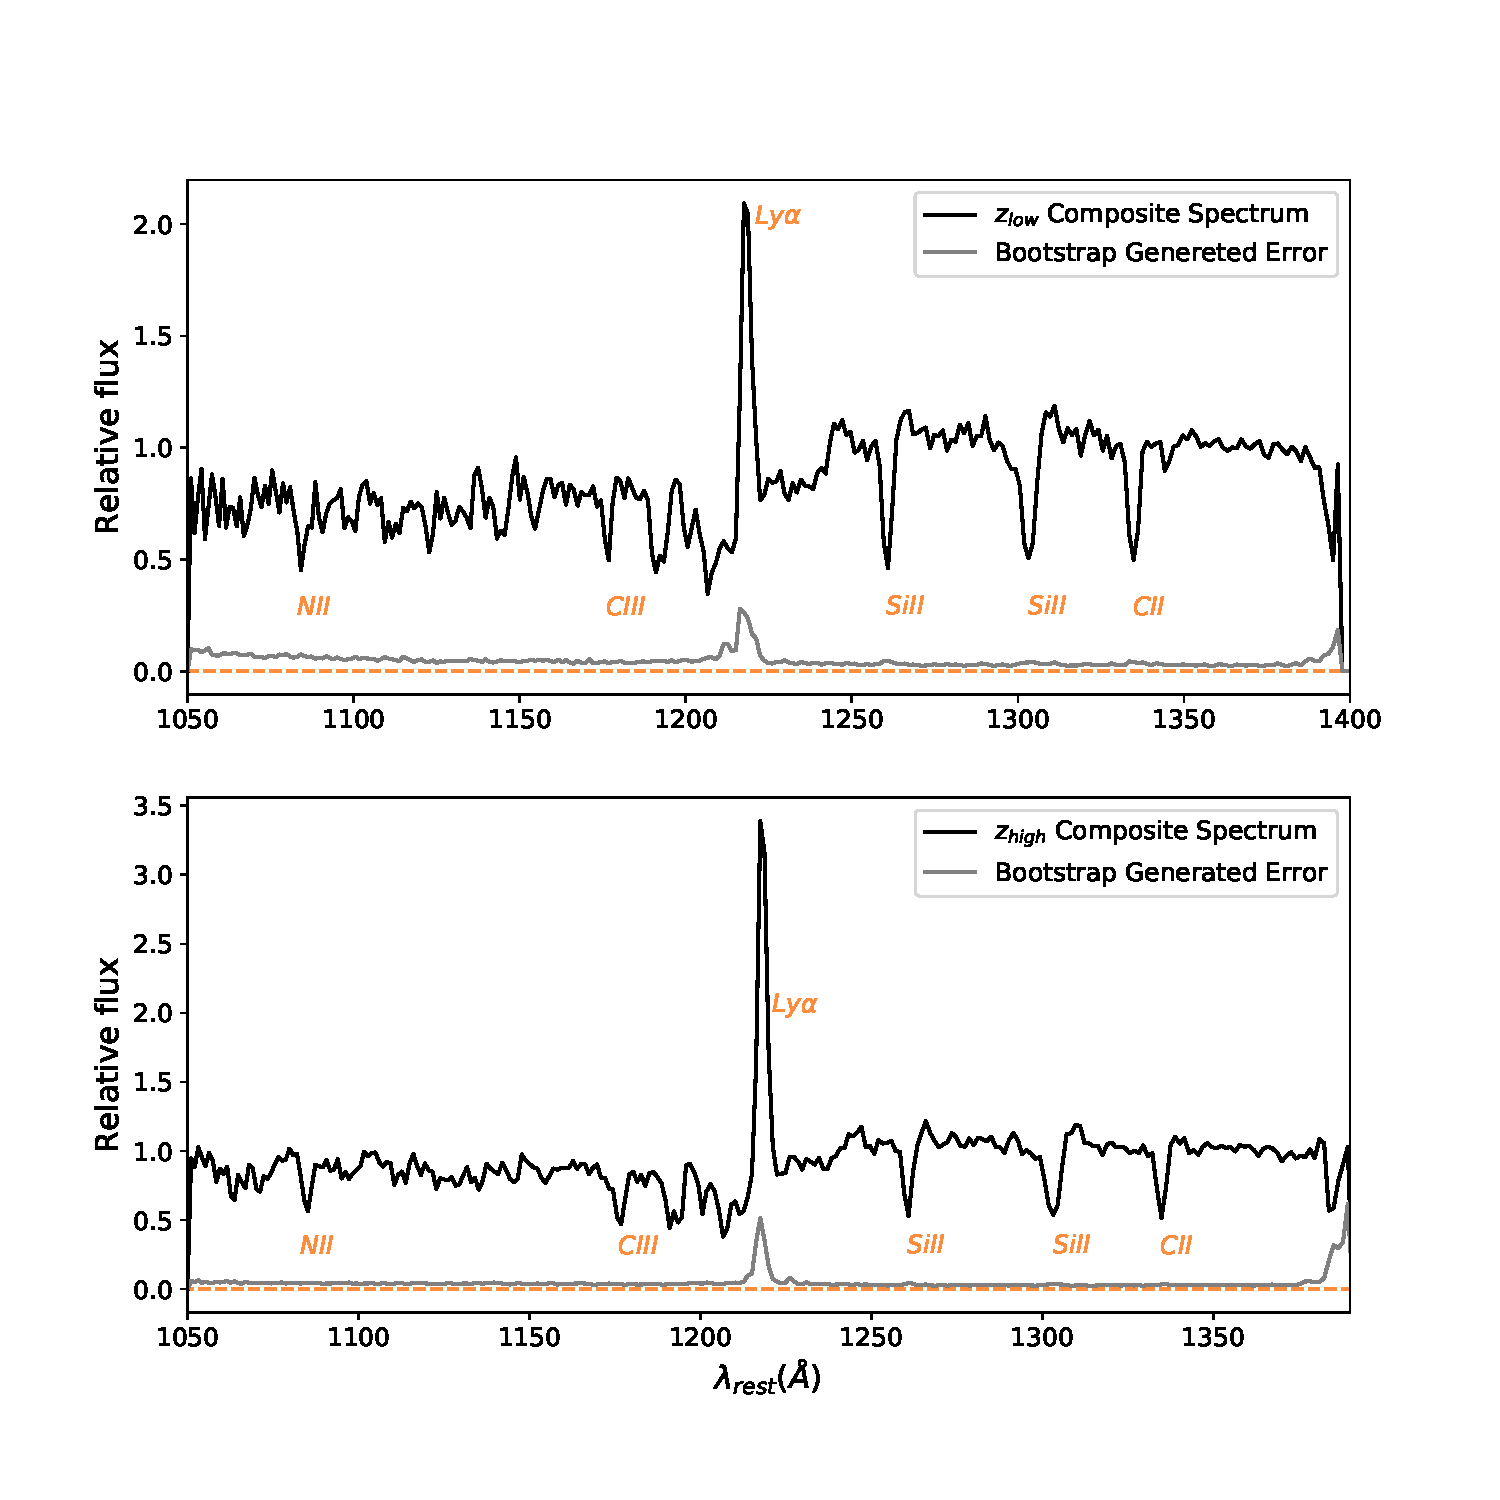
\includegraphics[scale = .5]{composites.pdf}
    \caption{The \loz and \hiz bin composite spectra with \zem = 2.44, 2.58, respectively. Here, the error spectrum is based on the bootstrap matrix (see \ref{subsec:bootstrap}) and not the CLAMATO values.}
    \label{fig:stack_1}
\end{figure*}

\section{SED Modeling}%%%%%%%%%%%%%%%%%%%%%%%%%%%%%%%%%%%%%%%%%%%%%%%%%%%%%%%%%%%%%%%

To measure \teff we estimate the unabsorbed flux of the composite spectrum in the \lya forest. We follow the examples of \cite{paris_principal_2011, prochaska_towards_2014} in that we estimate the unabsorbed continuum by extrapolating blueward of \lya into the forest. We used modules designed by John Chisholm that utlizes MPFIT, an IDL-based least-squares curve fitting program, to fit simple stellar population (SSPs) models to spectra using SSPs from the Starburst99 (SB99) database. \footnote{http://www.stsci.edu/science/starburst99/docs/} \citep{1999ApJS..123....3L}.

There are 50 SB99 models of a single star at a single age and a single stellar metallicity. We explore 10 stellar ages in our models: 1, 2, 3, 4, 5, 8, 10, 20, 40 Myr, each with 5 different metallicities: 0.05, 0.2, 0.4, 1.0, 2.0 $Z_\odot$. Each model is fully theoretical and was created by sampling the high-mass portion of the Hertzsprung-Russell diagram up to temperatures of 20,000 K. 

Our fitting routine is based on two best fit parameters; the fraction of light multiplied by each stellar continuum model $\mathrm{L_{frac}}$ and the attenuation parameter E(B-V). The parameter $\mathrm{L_{frac}}$ is reported for any of the 50 SB99 models that go into making the final fit while the E(B-V) parameter is a single value used to redden the fit. Using the $\mathrm{L_{frac}}$ values for the models, we can estimate the age and the metalicity of the source (see table \ref{tab:params}).

\begin{figure*}[ht]
    \centering
    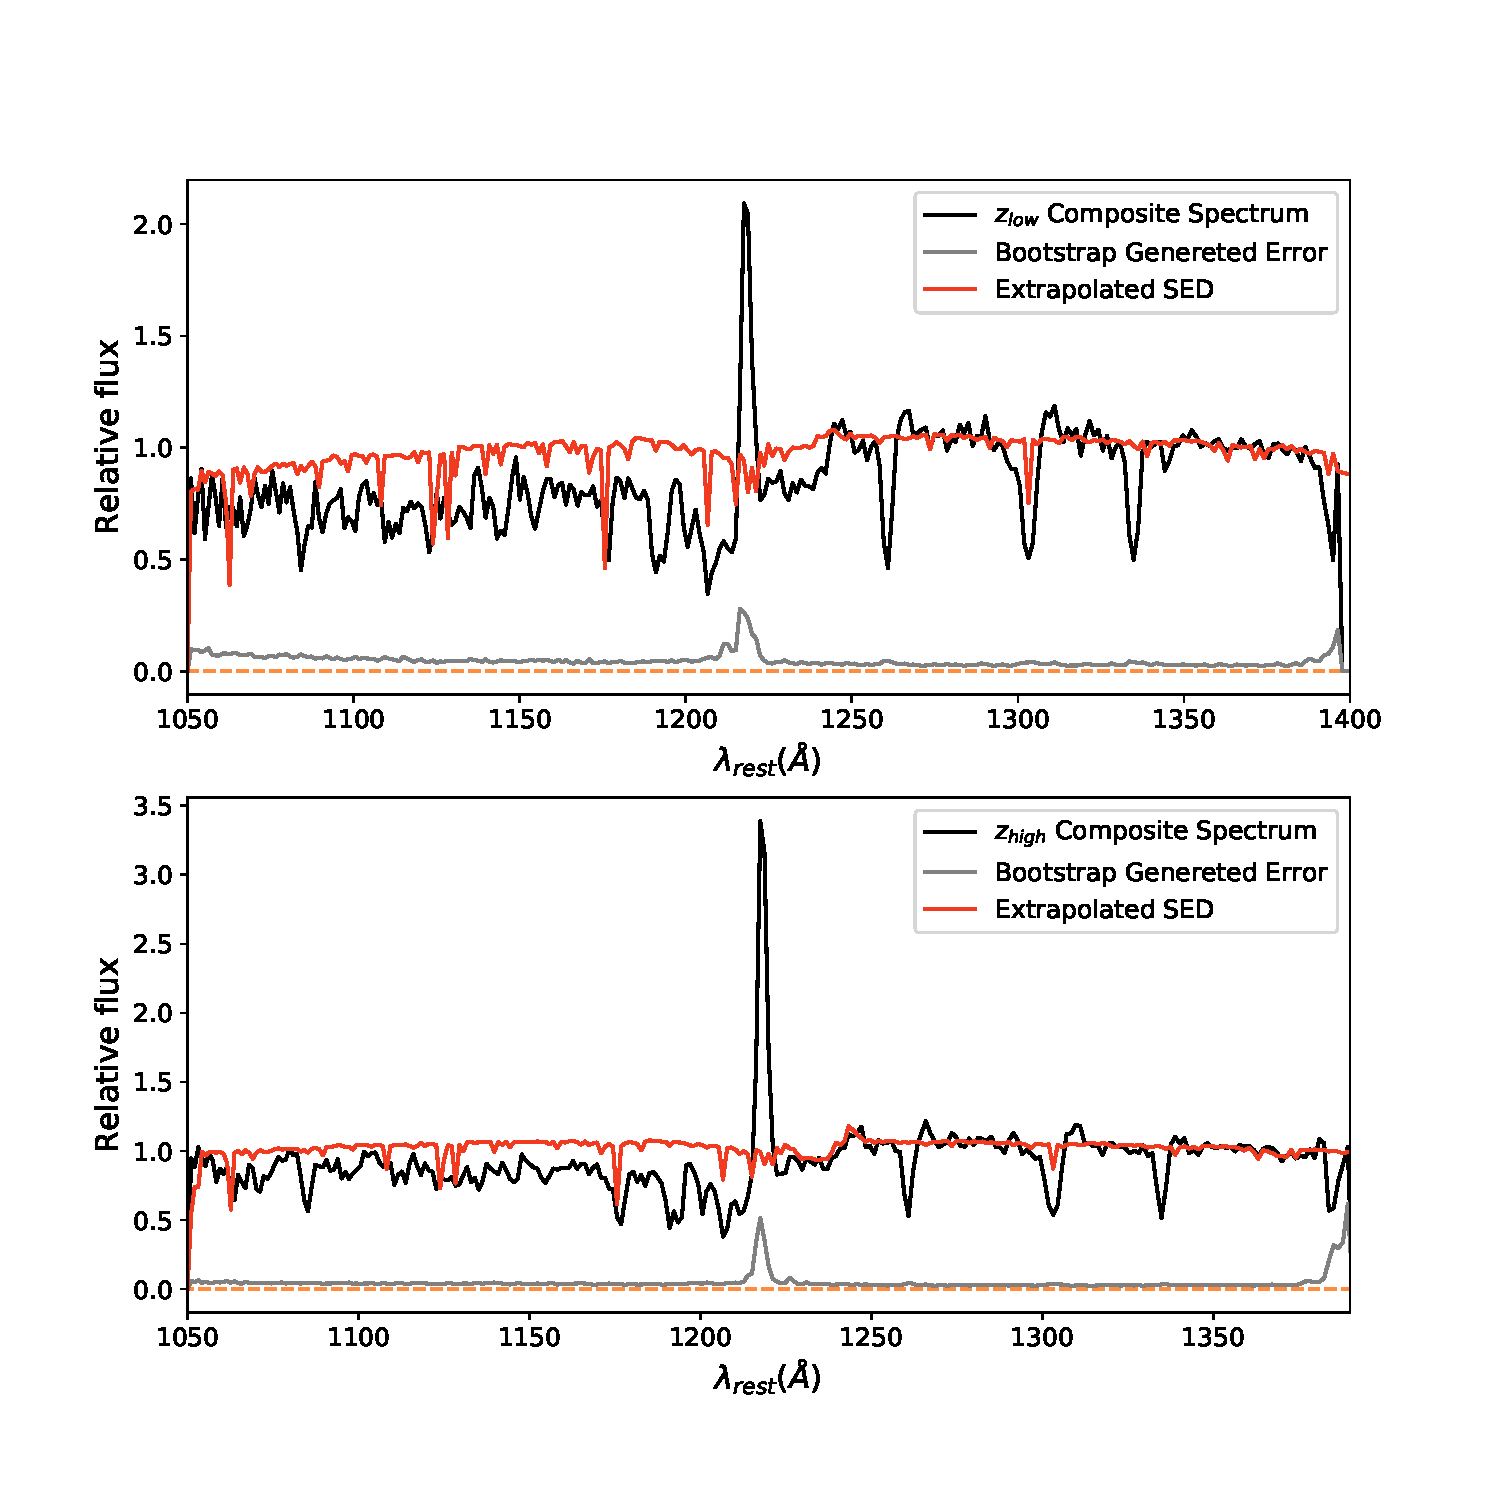
\includegraphics[scale = .5]{models.pdf}
    \caption{The composite spectra plotted in black and their SED fits are plotted in red. The discrepancy in blue-ward of \lya illustrates where the HI is attenuating the spectrum and therefore the range in which we measure \teff.}
    \label{fig:model}
\end{figure*}

Following the procedure written by \cite{chisholm_constraining_2018} to fit these models to our data, we start by masking out 23 different ISM absorption lines ($\pm$ 500 \kms) that would otherwise contaminate the fitting. Then we fit only within the wavelength range of 1225\AA - 1400\AA, to take advantage of the unattenuated section of the spectrum redward of \lya. By inputting the bootstrap-generated error array (S/N $\sim 10$) we are able to model a a smooth continuum into the \lya forest. Then, using the attenuation curve from \cite{reddy_spectroscopic_2016}, we redden our fitting results and normalize them in the same range as the composites. Finally, we rebin them to a matching velocity dispersion of 300\kms. 


\begin{table*}[ht]
\begin{center}
\caption{MPFIT Parameters}
\label{tab:params}
\vskip0.1in
\begin{tabular}{cccc}
\hline
\hline
Redshift Bin & Age (Myr) & Metalicity ($Z_\odot$) & E(B-V)\\
\hline
$2.442$ (\loz) & $8.977$ & $0.148$ & $0.268 \pm 0.013$\\
$2.606$ (\hiz) & $5.320$ & $0.074$ & $0.229 \pm 0.014$\\
\hline
\end{tabular}
\end{center}
\end{table*}

We assess the quality of the modeled SEDs based on two characterisitics. First, how closely the model matches the absorbed continuum in the fitting region from 1225\AA - 1500\AA\space and second, whether the model stays consistently higher than the absorbed continuum in the \lya forest. To report errors on the fitting process and because these two characteristics are not readily quantifiable (apart of visual inspection), we ran our 10,000 randomized composites from the bootstrap analysis through the fitting process creating a distribution of SEDs which we propagate through to our analysis of \teff (see \ref{subsec:errors}).


\section{Analysis} %%%%%%%%%%%%%%%%%%%%%%%%%%%%%%%%%%%%%%%%%%%%%%%
\label{sec:Effective Opacity Measurements}

Armed with the bootstrap generated composite spectra, and a corresponding SED for each realization, we analyze the \lya forest to measure an effective opacity for each wavelength index ($\lambda_{i}$). For each composite, we mask out the following ISM lines $1083.99, 1117.97, 1122.52, 1128.01, 1144.93, 1152.81 \AA$ $\pm$ a $5\AA$ buffer. Then, using equation \ref{eq1}, we covert the wavelength array to values of redshift $z_{i}$.

\begin{equation}
        z_{i} = (\lambda_{i}/\lambda_{1216})(1 + z_{med}) - 1
        \label{eq1}
\end{equation}

Combining both redshift bins, we are left with a total of $88 \lambda_{i}$ bins from which to measure \teff in the \lya forest (1070-1170\AA). However, because the \zem values of the two bins are similar, their redshift coverage often overlaps. (See tables \ref{tab:lowz_tab} and \ref{tab:hiz_tab}). Next, we use the equation \ref{eq2} to measure the effective opacity for every composite/SED model pair. $F_{obs}$ is the composite flux value, $F_{model}$ is the extrapolated SED flux value and $z_{i}$ is the redshift of a specific $\lambda_{i}$.

\begin{equation}
        \tau_{eff} = -\ln \frac{F_{\rm obs}}{F_{\rm model}}
        \label{eq2}
\end{equation}

We define the median value per redshift bin $z_{i}$ (across the bootstrap grid) as our measurements of the effective opacity of HI.

\subsection{Errors}
\label{subsec:errors}

The errors on the \teff values ($\sigma_{\tau}$) are directly measured from the bootstrap analysis but are not simply the standard deviation of each redshift bin across the bootstrap. Instead, we calculate the covariance matrix across our redshift bins and feed the full (Nbin x Nbin) matrix into our least-squares power-law fitting and published literature comparisons (see sections \ref{subsec:evo} and  \ref{sec:conclusions}).

There is no uncertainty in the redshift values we report in tables \ref{tab:lowz_tab} and \ref{tab:hiz_tab}, as they are only dependant on the \zem and $\lambda_{i}$, neither of which have corresponding errors. Because both bins have the same size ($\Delta$z $\sim$ 0.25) and similar distributions, we mitigate any uncertainty in \zem.

\subsection{Redshift Evolution} %%%%%%%%%%%%%%%%%%%%%%%%%%%%%%%%%%%%%%%%%%%%%%%%%%%%%%%%%
\label{subsec:evo}

Using a least-squares formalism, we fit our measurements of \teff, with the following analytic power-law function. 

\begin{center}
\begin{equation}
        \tau_{eff} = A[(1+z)/(1+z_{med})]^{B}
        \label{eq4}
\end{equation}
Where A and B are the scale factor and power-law index parameters. The \zem value included in the function acts as a pivot: essentially normalizing the values of \teff. We take \zem $\equiv 2.32$.
\end{center}

We report a \rchi value of 1.941 with 86 degrees of freedom (DoF). Our best fit scale factor and power-law index parameters of A = $0.158 \pm 0.007$ and B = $0.493 \pm 1.114$ respectively.

\begin{figure*}[ht]
    \centering
    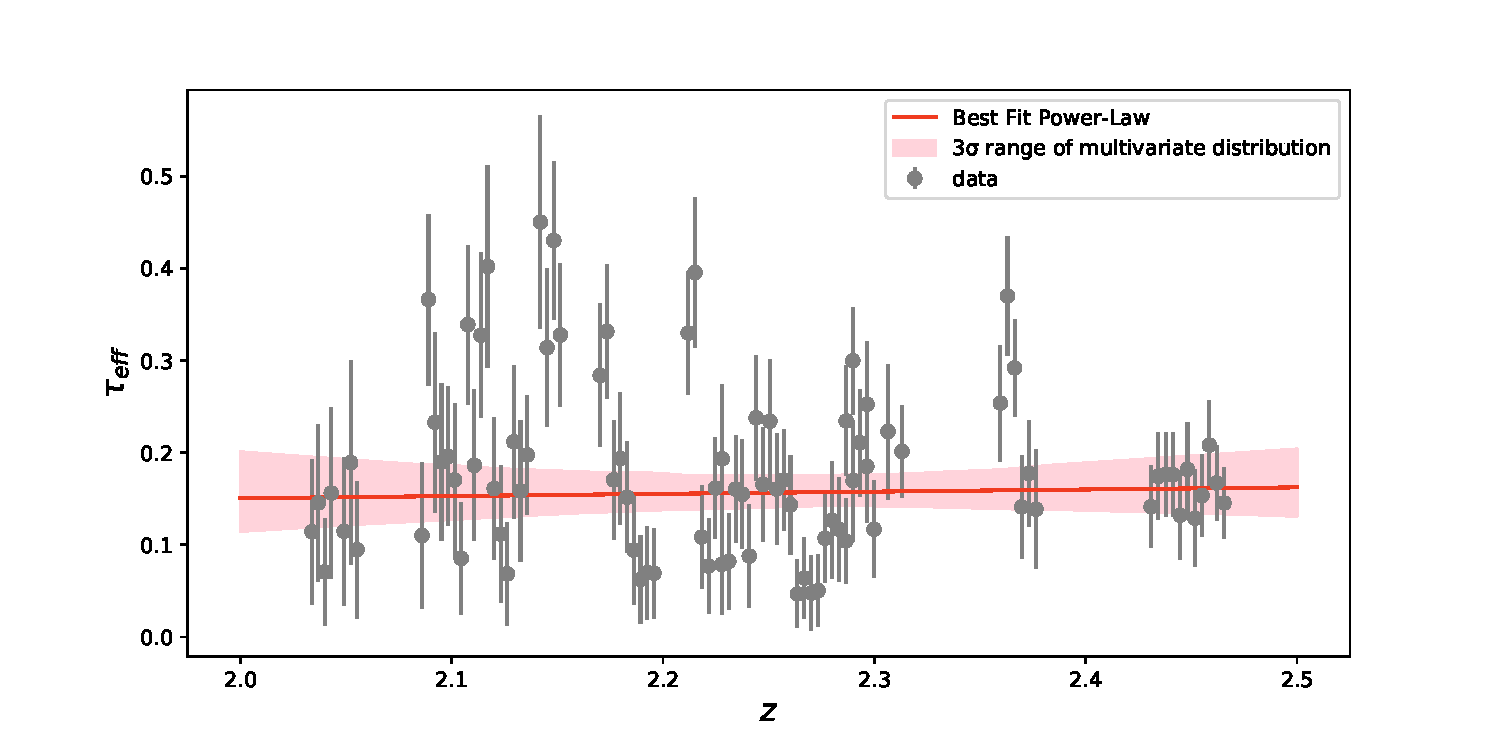
\includegraphics[scale = .5]{redshift_evolution.pdf}
    \caption{The results from equations \ref{eq1} and \ref{eq2}. The x-axis is rest-frame redshift and the y-axis is \teff. Both bins are plotted in grey and contribute to a wide range of values. The best fit line is plotted in red and has a \rchi value of 1.941 . The pink lines describe a 99.7 \% uncertainty in our scale and power-index parameters. Though the full covariance matrix was used to calculate the best fit, we only plot the 1D errors in tables \ref{tab:lowz_tab} and \ref{tab:hiz_tab}}
    \label{fig:scattertau}
\end{figure*}

\section{Conclusions}
\label{sec:conclusions}

\begin{figure*}[ht]
    \centering
    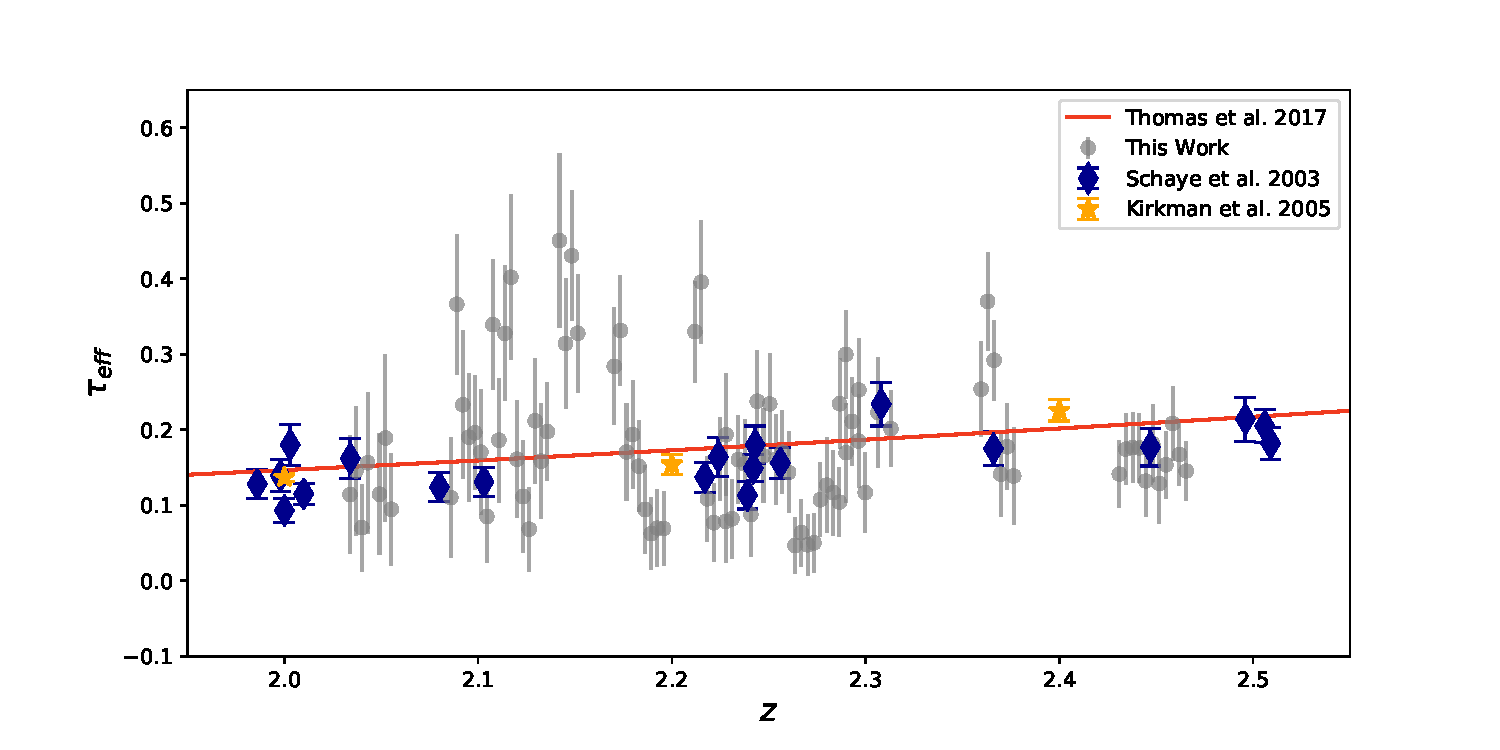
\includegraphics[scale = .5]{comptau.pdf}
    \caption{Here is our data compared to other works \cite{thomas_vimos_2017, schaye_metallicity_2003, kirkman_h_2005}. We sport a scattered distribution in our "narrow" range ($\Delta z$ $\sim$ 0.4) making it hard to contrain the evolution of \teff}
    \label{fig:comptau}
\end{figure*}

1) By stacking galaxies that are not at the same redshift, we sample \lya forests that are attenuated in different ways \cite{1965ApJ...142.1633G}. This is relevant because stacking is essentially an average and is therefore susceptible to being skewed by "outliers" (of which we have many especially in the \lya forest). A remedy would be to study a much larger sample to include several more galaxy spectra in the stacks. 

2) The process we used to fit our composites is an educated extrapolation into a noisy section of our composite spectra. Though we extrapolate using the bootstrap-generated errors from a well behaved portion of the spectra (red-ward of \lya), the models we use are calculated from the single age populations. We used this modelling technique mainly because it was readily available to us. In the future we could explore a more sophisticated method of SED modelling, such as PCA \citep{paris_principal_2011, Suzuki_2006}

3) Our estimate of the redshift evolution are not especially insightful mainly because both bins produced a scattered distribution of \teff values, many of which we expect to be nonphysical. We do however, recognize that our data does not contradict seminal studies. \cite{thomas_vimos_2017, faucher-giguere_direct_2008, becker_refined_2013} all fit similar power law functions to their data based on theories from \cite{1965ApJ...142.1633G}. Comparing their predictions at our redshifts, we report \rchi = 2.125 with 86 DoF for \cite{thomas_vimos_2017}, \rchi = 2.348 with 86 DoF for \cite{faucher-giguere_direct_2008}, and \rchi = 2.216 with 85 DoF for \cite{becker_refined_2013}.

4) Our analysis confirms that the accepted predictions for the evolution of \teff at lower redshifts are well constructed. We plot our results against similar measurements from \cite{schaye_metallicity_2003, kirkman_h_2005} along with the published literature model that agrees best with our data, \cite{becker_refined_2013}.

\begin{acknowledgements}
Jose Monzon would like to thank Sunil Simha, Marie Lau, Jiani Ding, Rion Parsons, John Chisholm and Khee-Gan Lee for their guidance and input with several aspects of this project. He would also like to thank Professor Prochaska for his invaluable support and mentorship
\end{acknowledgements}

\newpage

\begin{table*}
\parbox{.45\linewidth}{
\centering
\caption{\teff values for the \loz redshift bin. The $\sigma_{\tau}$ values here are simply the square root of the diagonal indices of our covariance matrix.}
\label{tab:lowz_tab}
\vskip0.1in
\begin{tabular}{ccc}
\hline
\hline
$z$ & \teff & $\sigma_{\tau}$\\
\hline
2.034 & 0.114 & 0.082 \\
2.037 & 0.146 & 0.086 \\
2.04 & 0.07 & 0.064 \\
2.043 & 0.156 & 0.094 \\
2.049 & 0.115 & 0.083 \\
2.052 & 0.189 & 0.111 \\
2.055 & 0.095 & 0.082 \\
2.086 & 0.11 & 0.084 \\
2.089 & 0.366 & 0.093 \\
2.092 & 0.233 & 0.098 \\
2.095 & 0.19 & 0.085 \\
2.098 & 0.196 & 0.076 \\
2.101 & 0.17 & 0.083 \\
2.104 & 0.085 & 0.064 \\
2.108 & 0.339 & 0.086 \\
2.111 & 0.186 & 0.082 \\
2.114 & 0.328 & 0.089 \\
2.117 & 0.402 & 0.109 \\
2.12 & 0.161 & 0.077 \\
2.123 & 0.112 & 0.076 \\
2.126 & 0.068 & 0.061 \\
2.129 & 0.212 & 0.083 \\
2.133 & 0.158 & 0.076 \\
2.136 & 0.198 & 0.065 \\
2.142 & 0.45 & 0.116 \\
2.145 & 0.314 & 0.086 \\
2.148 & 0.43 & 0.086 \\
2.151 & 0.328 & 0.078 \\
2.212 & 0.33 & 0.067 \\
2.215 & 0.396 & 0.081 \\
2.218 & 0.108 & 0.056 \\
2.222 & 0.077 & 0.053 \\
2.225 & 0.162 & 0.055 \\
2.228 & 0.193 & 0.081 \\
2.283 & 0.117 & 0.057 \\
2.287 & 0.234 & 0.06 \\
2.29 & 0.17 & 0.066 \\
2.297 & 0.253 & 0.068 \\
2.3 & 0.117 & 0.053 \\
2.306 & 0.223 & 0.073 \\
2.313 & 0.201 & 0.05 \\
\hline
\end{tabular}
}
\hfill
\parbox{.45\linewidth}{
\centering
\caption{\teff values for the \hiz redshift bin. The $\sigma_{\tau}$ values here are simply the square root of the diagonal indices of our covariance matrix.}
\label{tab:hiz_tab}
\vskip0.1in
\begin{tabular}{ccc}
\hline
\hline
$z$ & \teff & $\sigma_{\tau}$\\
\hline
2.17 & 0.284 & 0.078 \\
2.173 & 0.332 & 0.073 \\
2.177 & 0.171 & 0.065 \\
2.18 & 0.194 & 0.071 \\
2.183 & 0.152 & 0.06 \\
2.186 & 0.094 & 0.059 \\
2.189 & 0.062 & 0.053 \\
2.193 & 0.07 & 0.053 \\
2.196 & 0.069 & 0.051 \\
2.228 & 0.079 & 0.058 \\
2.231 & 0.082 & 0.053 \\
2.234 & 0.16 & 0.058 \\
2.238 & 0.155 & 0.059 \\
2.241 & 0.088 & 0.057 \\
2.244 & 0.238 & 0.068 \\
2.247 & 0.165 & 0.062 \\
2.251 & 0.234 & 0.067 \\
2.254 & 0.161 & 0.06 \\
2.257 & 0.17 & 0.055 \\
2.26 & 0.143 & 0.054 \\
2.264 & 0.047 & 0.041 \\
2.267 & 0.064 & 0.046 \\
2.27 & 0.048 & 0.043 \\
2.273 & 0.05 & 0.043 \\
2.277 & 0.107 & 0.049 \\
2.28 & 0.127 & 0.063 \\
2.286 & 0.104 & 0.046 \\
2.29 & 0.3 & 0.058 \\
2.293 & 0.211 & 0.058 \\
2.296 & 0.185 & 0.061 \\
2.36 & 0.254 & 0.063 \\
2.363 & 0.37 & 0.065 \\
2.366 & 0.292 & 0.053 \\
2.37 & 0.141 & 0.056 \\
2.373 & 0.177 & 0.057 \\
2.376 & 0.139 & 0.064 \\
2.431 & 0.141 & 0.045 \\
2.434 & 0.174 & 0.047 \\
2.438 & 0.177 & 0.046 \\
2.441 & 0.176 & 0.046 \\
2.445 & 0.132 & 0.048 \\
2.448 & 0.182 & 0.051 \\
2.452 & 0.129 & 0.053 \\
2.455 & 0.153 & 0.044 \\
2.458 & 0.208 & 0.049 \\
2.462 & 0.167 & 0.041 \\
2.465 & 0.145 & 0.039 \\
\hline
\end{tabular}
}
\end{table*}

\bibliography{IGM_refs.bib}

\end{document}
  
  
 